\documentclass[fontset=windows,12pt]{article}

\usepackage[UTF8]{ctex}
\usepackage[a4paper]{geometry}
\usepackage{amsmath}
\usepackage{fancyhdr}
\usepackage{amsthm}
\usepackage{amssymb}
\usepackage{xcolor}
\usepackage{listings}
\usepackage{graphicx}
\usepackage{circuitikz}
\usepackage{tikz,xcolor} % 绘制图形和使用颜色的宏包
\usepackage{multicol} % 多栏排版的宏包
\usepackage{multirow} % 表格中合并单元格的宏包
\usepackage{pdfpages} % 插入PDF文件的宏包
\RequirePackage{listings} % 在文档中插入源代码的宏包
\RequirePackage{xcolor} % 定义和使用颜色的宏包
\usepackage{wrapfig} % 文字绕排图片的宏包
\usepackage{bigstrut,multirow,rotating} % 支持在表格中使用特殊命令的宏包
\usepackage{booktabs} % 创建美观的表格的宏包
\usepackage{circuitikz} % 绘制电路图的宏包
\usepackage{xeCJK} 
\usepackage[table]{xcolor}  
\usepackage{multirow}
\usepackage{diagbox}
\usepackage{slashbox}
\newcolumntype{C}[1]{>{\centering\arraybackslash}p{#1}} %定义居中的列
\ctikzset{logic ports=ieee}     %所有逻辑门使用IEEE标准
\usetikzlibrary{calc}           %使用TikZ中的计算功能
\setlength{\headheight}{14.49998pt}

\newtheorem{question}{\hskip 1.7mm \bf}
\renewenvironment{proof}{{\noindent\hskip 2em \bf ֤证明 \quad}}{\hfill$\qed$\par}
\newenvironment{solution}{{\noindent\hskip 2.4em \bf 解 \quad}}

\geometry{left=2.0cm,right=2.0cm,top=2.5cm,bottom=2.5cm}
\begin{document}

\definecolor{CPPLight}  {HTML} {686868}
\definecolor{CPPSteel}  {HTML} {888888}
\definecolor{CPPDark}   {HTML} {262626}
\definecolor{CPPBlue}   {HTML} {4172A3}
\definecolor{CPPGreen}  {HTML} {487818}
\definecolor{CPPBrown}  {HTML} {A07040}
\definecolor{CPPRed}    {HTML} {AD4D3A}
\definecolor{CPPViolet} {HTML} {7040A0}
\definecolor{CPPGray}  {HTML} {B8B8B8}
\lstset{
    columns=fixed,       
    numbers=left,                                        % 在左侧显示行号
    frame=none,                                          % 不显示背景边框
    backgroundcolor=\color[RGB]{245,245,244},            % 设定背景颜色
    keywordstyle=\color[RGB]{40,40,255},                 % 设定关键字颜色
    numberstyle=\footnotesize\color{darkgray},           % 设定行号格式
    commentstyle=\it\color[RGB]{0,96,96},                % 设置代码注释的格式
    stringstyle=\rmfamily\slshape\color[RGB]{128,0,0},   % 设置字符串格式
    showstringspaces=false,                              % 不显示字符串中的空格
    language=verilog,                                        % 设置语言
    morekeywords={default,reg,wire,assign,module,endmodule,always,input,output,alignas,continute,friend,register,true,alignof,decltype,goto,
    reinterpret_cast,try,asm,defult,if,return,typedef,auto,delete,inline,short,
    typeid,bool,do,int,signed,typename,break,double,long,sizeof,union,case,
    dynamic_cast,mutable,static,unsigned,catch,else,namespace,static_assert,using,
    char,enum,new,static_cast,virtual,char16_t,char32_t,explict,noexcept,struct,
    void,export,nullptr,switch,volatile,class,extern,operator,template,wchar_t,
    const,false,private,this,while,constexpr,float,protected,thread_local,xnor,
    const_cast,for,public,throw,std},
    emph={map,set,multimap,multiset,unordered_map,unordered_set,
    unordered_multiset,unordered_multimap,vector,string,list,deque,
    array,stack,forwared_list,iostream,memory,shared_ptr,unique_ptr,
    random,bitset,ostream,istream,cout,cin,endl,move,default_random_engine,
    uniform_int_distribution,iterator,algorithm,functional,bing,numeric,begin,end},
    emphstyle=\color{CPPViolet}, 
}
\newenvironment{correction}{\par\noindent{\color{blue}{\bf{更正\\}}}\quad\color{blue}}{\par}
\pagestyle{fancy}
\lhead{中国科学院大学}
\chead{\bf{2024-25秋数字电路课程}}
\rhead{\emph{2023K8009929044 薛翼舟}}


\begin{center}
\huge{\bf{实验3 状态机实验}}
\end{center}

\section{实验目的}
    \subsection{熟悉verilog编程与调试}
    \subsection{熟悉状态机的工作原理, 能熟练编写状态机程序}




\section{实验环境}
    AMD Vivado2022.2





\section{原理说明}
    在本次实验课中, 主要学习了在verilog中编写状态机程序, 一般采用三段式来编写状态机程序, 也即
    \begin{enumerate}
        \item 阻塞的异步置数以及状态转换
        \item 根据输入和当前状态产生下一状态
        \item 根据输入和当前状态产生输出
    \end{enumerate}
    在本实验中, 并未设计比较有挑战性或者创造性的电路, 因此在本次报告原理说明的部分主要内容是状态转移图以及思路讲解
    \subsection{序列检测器}
        两个序列检测器都能够检测重叠序列, 只需要改变状态转移即可, 在设计可检查重叠序列的序列检测器中, 要注意状态转移图中, 最后输出为1的状态
        再次接受输入后的状态转移并非回到初始, 而是根据子序列返回到之前某个状态中, 两个状态转移图如下
        \begin{figure}[ht]
            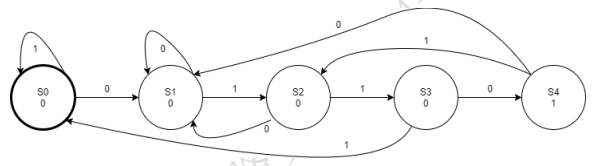
\includegraphics[width=0.6\textwidth]{转移图1.jpg}
            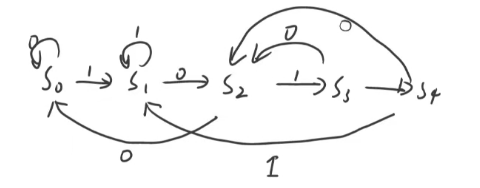
\includegraphics[width=0.4\textwidth]{转移图2.jpg}
            \caption{左:0110的序列检测\qquad 右:1011的序列检测}
        \end{figure}


    \subsection{周期性输出}
        本次实验中, 采用了最简单的状态周期转移构成的12计数器, 只不过是改变了中间某些状态的输出, 不只是在最终状态的输出
        主要是$S_0\sim S_{11}$共12个状态, 一个时钟周期转换一个状态, 每个周期输出相应的输出
        在本实验中的状态转移图是简单的线性, 并无较大的参考价值, 在这里直接画出状态转移表
        \begin{table}[ht]
            \centering
            \begin{tabular}{|C{2.1cm}|C{1.1cm}C{1.1cm}C{1.1cm}C{1.1cm}|C{1.1cm}|}\hline
                时钟周期 & \multicolumn{4}{|c|}{电路状态} & 输出 \\\hline
                clk & $S_3$ & $S_2$ & $S_1$ & $S_0$ & Y \\\hline
                0 & 0 & 0 & 0 & 0 & 0\\
               \rowcolor{gray!25} 1 & 0 & 0 & 0 & 1 & 0\\
                2 & 0 & 0 & 1 & 0 & 0\\
                \rowcolor{gray!25}3 & 0 & 0 & 1 & 1 & 0\\
                4 & 0 & 1 & 0 & 0 & 0\\
                \rowcolor{gray!25}5 & 0 & 1 & 0 & 1 & 0\\
                6 & 0 & 1 & 1 & 0 & 0\\
                \rowcolor{gray!25}7 & 0 & 1 & 1 & 1 & 0\\
                8 & 1 & 0 & 0 & 0 & 0\\
                \rowcolor{gray!25}9 & 1 & 0 & 0 & 1 & 0\\
                10 & 1 & 0 & 1 & 0 & 0\\
                \rowcolor{gray!25}11 & 1 & 0 & 1 & 1 & 1\\
                12 & 0 & 0 & 0 & 0 & 0\\\hline
            \end{tabular}
        \end{table}
    

    \subsection{报纸贩卖机}
        在本实验中采用的是当投入的币的金额超过5时, 直接reset, 输出为1当且仅当正好金额为5, 这个实验主要需要注意状态的转换, 状态转移图如下
        \begin{figure}[ht]
            \centering
            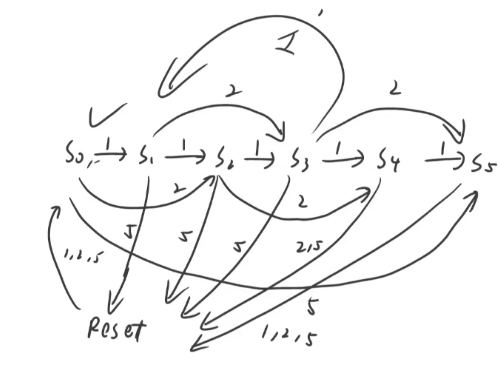
\includegraphics[width=0.4\textwidth]{转移图3.jpg}
            \caption{报纸贩卖机的状态转移图}
        \end{figure}






\section{接口定义}
    在本次实验的每一个程序之中, 内部都利用parameter或者localmeter来定义了几个状态常量, 另外有两个内部的接线状态state以及next\_state, 分别
    表示当前状态以及下一状态, 下面是每一个接口
    \subsection{序列检测器}
        两个序列检测器的接口完全相同, 不同的二者的状态转移, 详见源代码部分
        {\setmainfont{Courier New Bold}                               
        \begin{lstlisting}
    input clk,              \\时钟的输入
    input in,               \\输入
    input rstn,             \\异步置数的输入
    output reg out          \\输出, 因为在always中赋值, 需要使用reg
        \end{lstlisting}}
   \subsection{周期性输出}
        {\setmainfont{Courier New Bold}                               
        \begin{lstlisting}
    input clk,              \\时钟的输入
    input rstn,             \\异步置数, 此程序不需要输入
    output reg out          \\输出
        \end{lstlisting}}
    \subsection{报纸贩卖机}
    {\setmainfont{Courier New Bold}                               
    \begin{lstlisting}
    input [1:0]in,          \\因为有1,2,5三个输入, 因此需要2位输入
    input clk,              \\时钟的输入
    input rstn,             \\异步置数
    output reg out          \\输出
    \end{lstlisting}}





\section{调试过程以及结果}
    本次实验比较顺畅, 并未出现较大的困难, 相比于实验2.5给出的代码, 本次实验在代码中的状态转移并没有使用if-else语句来描述, 而是利用了
    cases的嵌套, 个人认为这样的代码更加简洁, 而且可读性更高.\par
    另外, 一个比较明显的困难是在随机数0,1,2的生成, 由于verilog中random()语句生成的随机数是有符号的, 因此\$random() \% 2 会生成显示为3的-1,
    因此这里需要随机生成无符号数, 经过资料查找, 该效果可以用语句\$urandom\_range(2, 0);来实现
    \subsection{序列检测器}
        \subsubsection{0110序列检测}
        \begin{figure}[ht]
            \centering
            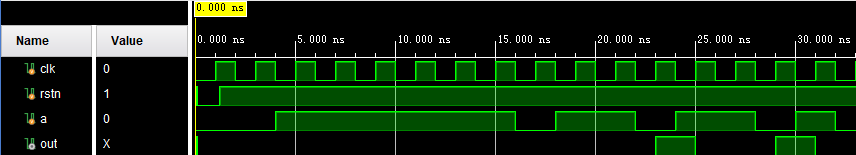
\includegraphics[width=1\textwidth]{波形图1.jpg}
            \caption{0110序列检测器的波形图}
        \end{figure}
        \subsubsection{1011序列检测器}
        \begin{figure}[ht]
            \centering
            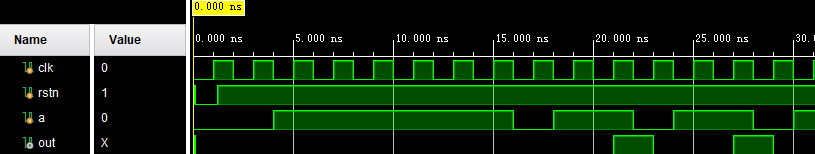
\includegraphics[width=1\textwidth]{波形图2.jpg}
            \caption{1011序列检测器的波形图}
        \end{figure}
        \subsection{周期输出序列}
        \begin{figure}[ht]
            \centering
            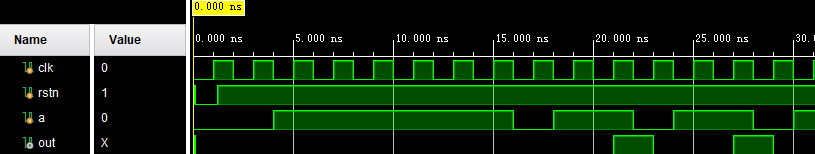
\includegraphics[width=1\textwidth]{波形图2.jpg}
            \caption{周期输出序列波形图}
        \end{figure}
        \bigskip\bigskip\bigskip\bigskip\bigskip\bigskip\bigskip\bigskip\bigskip\bigskip\bigskip\bigskip\bigskip\bigskip
        \subsection{报纸贩卖机波形图}
        \begin{figure}[ht]
            \centering
            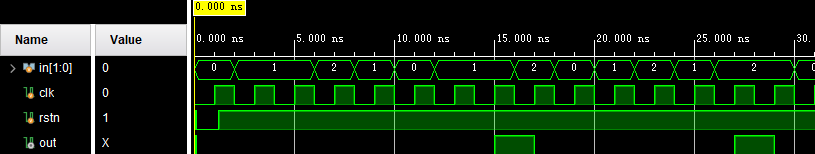
\includegraphics[width=1\textwidth]{波形图4.jpg}
            \caption{报纸贩卖机波形图}
        \end{figure}




\section{实验总结}
    经过本次实验, 极大程度上达成了实验目的, 熟练掌握了三段式状态机的工作以及编写原理, negedge和posedge分别表示下降, 上升沿触发同时对与testbench的编写有了更加深刻的体会, 比如clk的编写, 初始化输入以及异步置数等, 
    了另外对于testbench中的随机数生成有了使用\$urandom\_range(m, n);的办法



\section{源代码}
    由于本次实验的testbench比较重要, 因此本次报告中的源代码部分分为设计文件和激励文件两部分
    \subsection{设计文件}
        \subsubsection{0110序列检测}
        {\setmainfont{Courier New Bold}                               
        \begin{lstlisting}
module check_str(
    input clk,
    input in,
    input rstn,
    output reg out
);
    parameter s0 = 3'b000;
    parameter s1 = 3'b001;
    parameter s2 = 3'b010;
    parameter s3 = 3'b011;
    parameter s4 = 3'b100;
    //无关状态
    parameter s5n = 3'b101;
    parameter s6n = 3'b110;
    parameter s7n = 3'b111;
    
    reg [2:0]state;
    reg [2:0]next_state;
    
    
    
    always @(negedge rstn or posedge clk)begin
        if(!rstn)begin
            state <= s0;
        end
        else begin
            state <= next_state;
        end
    end
        
        
        
    always @(state or in)begin
        case(state)
        s0:begin
            case(in)
            0 : next_state = s1;
            1 : next_state = s0;
            endcase
        end
        s1:begin
            case(in)
            0 : next_state = s1;
            1 : next_state = s2;
            endcase
        end
        s2:begin
            case(in)
            0 : next_state = s1;
            1 : next_state = s3;
            endcase
        end
        s3:begin
            case(in)
            0 : next_state = s4;
            1 : next_state = s0;
            endcase
        end
        s4:begin
            case(in)
            0 : next_state = s1;
            1 : next_state = s2;
        default: next_state=s0;
            endcase
        end
        endcase
    end
    
    

    always@(state)begin
        case(state)
        s0: out = 1'b0;
        s1: out = 1'b0;
        s2: out = 1'b0;
        s3: out = 1'b0;
        s4: out = 1'b1;
        default: out=1'bx;
        endcase
    end
    
endmodule
        \end{lstlisting}}
        \subsubsection{1011序列检测}
        {\setmainfont{Courier New Bold}                               
        \begin{lstlisting}
module check_str_1(
    input clk,
    input in,
    input rstn,
    output reg out
);
    parameter s0 = 3'b000;
    parameter s1 = 3'b001;
    parameter s2 = 3'b010;
    parameter s3 = 3'b011;
    parameter s4 = 3'b100;
    //无关状态
    parameter s5n = 3'b101;
    parameter s6n = 3'b110;
    parameter s7n = 3'b111;
    
    reg [3:0]state;
    reg [3:0]next_state;
    
    
    
    always @(negedge rstn or posedge clk)begin
        if(!rstn)begin
            state <= s0;
        end
        else begin
            state <= next_state;
        end
    end
        
        
        
    always @(state or in)begin
        case(state)
        s0:begin
            case(in)
            0 : next_state = s0;
            1 : next_state = s1;
            endcase
        end
        s1:begin
            case(in)
            0 : next_state = s2;
            1 : next_state = s1;
            endcase
        end
        s2:begin
            case(in)
            0 : next_state = s0;
            1 : next_state = s3;
            endcase
        end
        s3:begin
            case(in)
            0 : next_state = s2;
            1 : next_state = s4;
            endcase
        end
        s4:begin
            case(in)
            0 : next_state = s2;
            1 : next_state = s1;
        default: next_state=s0;
            endcase
        end
        endcase
    end
    
    

    always@(state)begin
        case(state)
        s0: out = 1'b0;
        s1: out = 1'b0;
        s2: out = 1'b0;
        s3: out = 1'b0;
        s4: out = 1'b1;
        default: out=1'bx;
        endcase
    end
    
endmodule
        \end{lstlisting}}
        \subsubsection{周期输出序列}
        {\setmainfont{Courier New Bold}                               
        \begin{lstlisting}
module periodic_output(
    input clk,
    input rstn,
    output reg out
    );
    
    parameter s0 = 4'b0000;
    parameter s1 = 4'b0001;
    parameter s2 = 4'b0010;
    parameter s3 = 4'b0011;
    parameter s4 = 4'b0100;
    parameter s5 = 4'b0101;
    parameter s6 = 4'b0110;
    parameter s7 = 4'b0111;
    parameter s8 = 4'b1000;
    parameter s9 = 4'b1001;
    parameter s10 = 4'b1010;
    parameter s11 = 4'b1011;
    parameter s12 = 4'b1100;
    parameter s13 = 4'b1101;
    parameter s14 = 4'b1110;
    parameter s15 = 4'b1111;
    
    reg [3:0]state;
    reg [3:0]next_state;
    
    always @(negedge rstn or posedge clk)begin
        if(!rstn)begin
            state <= s0;
        end
        else begin
            state <= next_state;
        end
    end
    

    always @(state)begin
        case(state)
            s0: next_state = s1;
            s1: next_state = s2;
            s2: next_state = s3;
            s3: next_state = s4;
            s4: next_state = s5;
            s5: next_state = s6;
            s6: next_state = s7;
            s7: next_state = s8;
            s8: next_state = s9;
            s9: next_state = s10;
            s10: next_state = s11;
            s11: next_state = s0;
            default: next_state = s0;
        endcase
    end
    
    
    
    always @(state)begin
        case(state)
            s0: out = 0;
            s1: out = 0;
            s2: out = 1;
            s3: out = 0;
            s4: out = 1;
            s5: out = 0;
            s6: out = 0;
            s7: out = 1;
            s8: out = 1;
            s9: out = 0;
            s10: out = 1;
            s11: out = 1;
            default: out = 1'bx;
        endcase
    end

endmodule
        \end{lstlisting}}
        \subsubsection{报纸贩卖机}
        {\setmainfont{Courier New Bold}                               
        \begin{lstlisting}
module newspaper_machine(
    input [1:0]in,
    input clk,
    input rstn,
    output reg out
    );
    
    reg [2:0]state;
    reg [2:0]next_state;
    
    parameter s0 = 3'b000;
    parameter s1 = 3'b001;
    parameter s2 = 3'b010;
    parameter s3 = 3'b011;
    parameter s4 = 3'b100;
    parameter s5 = 3'b101;
    parameter s6 = 3'b110;
    parameter reset = 3'b111;
    
    always @(negedge rstn or posedge clk)begin
        if(!rstn)begin
            state <= s0;
        end
        else begin
            state <= next_state;
        end
    end
    
    
    always @(in or state)begin//in中0,1,2分别表示1,2,5分钱
        case(state)
            s0:case(in)
                    2'b00: next_state = s1;
                    2'b01: next_state = s2;
                    2'b10: next_state = s5;
                endcase
            s1:case(in)
                    2'b00: next_state = s2;
                    2'b01: next_state = s3;
                    2'b10: next_state = reset;
                endcase
            s2:case(in)
                    2'b00: next_state = s3;
                    2'b01: next_state = s4;
                    2'b10: next_state = reset;
                endcase
            s3:case(in)
                    2'b00: next_state = s4;
                    2'b01: next_state = s5;
                    2'b10: next_state = reset;
                endcase
            s4:case(in)
                    2'b00: next_state = s5;
                    2'b01: next_state = reset;
                    2'b10: next_state = reset;
                endcase
            reset: next_state = s0;
            default: next_state = reset;
        endcase
    end
    
    always @(state) begin
        case(state)
            s5: out = 1;
            reset: out = 1'b0;
            default: out = 0;
        endcase
    end
    
endmodule
        \end{lstlisting}}


\subsection{激励文件}
    \subsubsection{序列检测器}
    {\setmainfont{Courier New Bold}                               
        \begin{lstlisting}
    module test_check_str(

    );
    
    reg clk;
    reg rstn;
    reg a;
    wire out;
    
    check_str check(
        .clk(clk),
        .rstn(rstn),
        .in(a),
        .out(out)
    );
    
    initial begin
        clk=0;
        rstn=1;
        a=0;
        #0.1 rstn=0;
        #1.1 rstn=1;
    end
    
    always begin
        #1 clk = ~clk;
    end
    
    always begin
        #2 a = $random() % 2;
    end
    
endmodule
        \end{lstlisting}}


    \subsubsection{周期输出序列}
    {\setmainfont{Courier New Bold}                               
        \begin{lstlisting}
module test_periodic_output(

);
    
reg clk;
reg rstn;
wire out;

periodic_output start(
    .clk(clk),
    .rstn(rstn),
    .out(out)
);

initial begin
    clk = 0;
    rstn = 1;
    #0.1 rstn = 0;
    #1.1 rstn = 1;
end

always begin
    #1 clk = ~clk;
end

endmodule
        \end{lstlisting}}
    \subsubsection{报纸贩卖机}
    {\setmainfont{Courier New Bold}                               
        \begin{lstlisting}
module check_newpaper_machine(
    );
    
reg [1:0]in;
reg clk;
reg rstn;
wire out;

newspaper_machine start(
    .clk(clk),
    .in(in),
    .rstn(rstn),
    .out(out)
);

initial begin
    clk = 0;
    in = 0;
    rstn = 1;
    #0.1 rstn = 0;
    #1.1 rstn = 1;
end

always begin
    #1 clk = ~clk;
end

always begin
    #2 in = $urandom_range(2, 0);
end

endmodule
        \end{lstlisting}}


\end{document}